\chapter{6. Vehicle and Control Tests}

In this chapter the control strategy is applied to the real scale PEV and an stability and robustness analysis is presented as well. Due to the possibility of controlling the PEV remotely (through the Bluetooth module and the Android app) two models were studied simultaneously. After the proper analysis and validation in MATLAB, the control strategy was implemented in the Arduino boards and the PEV was tested several times. Here the results of these tests are presented.

\section{Control Strategy Analysis}

The control strategy works in parallel with the dynamic model of the vehicle. It receives the sensor data as inputs; that information, along with with the gains and the actual speed of the vehicle, gives result to the output signal $M_{t}$ that tilts the vehicle.

Regarding the sensors, the rotary encoder in the rear wheel and the pair of inertial motion units provide the necessary data. The longitudinal speed given by the rotary encoder is used to calculate the gains of the model as well. The actuated motor is the tilting NIDEC motor, since the steering motor only responses to the driver's inputs and the handle bar motor only does the haptic feedback to the driver.

\begin{figure}[!h]
	\includegraphics[width=1\linewidth]{figs/06/strategy3}
	\caption{Workflow of the control strategy: input from IMU and output to tilting actuator}
	\label{strategy}
\end{figure}

\newpage
\subsection{Model Parameters}

To calculate the gains of the control strategy it is first needed to obtain or measure the \textbf{parameters to complete the dynamic model}. This includes the vehicle and the wheels variables: 

$\hspace{2cm} m \enspace L_{f} \enspace L_{r} \enspace I_{x} \enspace I_{z} \enspace C_{f} \enspace C_{r} \enspace \lambda_{f} \enspace \lambda_{r} \enspace ...$.

Therefore, the model presented in Chapter 3 needs to be calculated for the PEV characteristics. Both the vehicle with and without the driver were modelled in CAD software (Solidworks). By indicating the material of each body the necessary properties for the control model were extracted.

The geometrical parameters -- $h \enspace L_{f} \enspace L_{r} \enspace R_{wf}\enspace R_{wr}\enspace b$ -- were measured directly from the model. The dynamic parameters -- $m \enspace I_{x} \enspace I_{z} \enspace ...$ --, on the other side, were extracted from the mass properties.

\begin{table*}[h!]
\centering
	\begin{tabular}{l|cc|l|l}
	%\hline
	\textbf{Name}      &  \textbt{\begin{tabular}[c]{@{}l@{}}Driver\\ included\end{tabular}} & \textbt{\begin{tabular}[c]{@{}l@{}}No driver\\ included\end{tabular}}   & \textbf{Units}         & \textbf{Description}                                   \\
	\hline
	$m$                  & 115                       & 35                          & kg                     & Total mass of the vehicle                              \\
	$h$                 & 0.91                      & 0.36                        & m                      & Position of the center of gravity G on the z axis      \\
	$L_f$                & 0.718                     & 0.518                       & m                      & Distance from center of gravity to front axle          \\
	$L_r$               & 0.61                      & 0.81                        & m                      & Distance from center of gravity to rear axle           \\
	$m_f$               & 52.82                     & 21.35                       & kg                     & Mass supported by the front wheels                     \\
	$m_r$                & 62.18                     & 13.65                       & kg                     & Mass supported by the rear wheel                       \\
	$I_x$               & 25.14                     & 4.00                        & kg m^2				  & Vehicle roll moment of inertia                         \\
	$I_z$                & 17.8                      & 10.93                       & kg m^2				  & Vehicle yaw moment of inertia                          \\
	$I_{wheel\,f\,\theta}$ & 0.05                      & 0.05                        & kg m^2				  & Tilting inertia of each front wheel about its own axis \\
	$I_{wheel\,f\,rot}$  & 0.11                      & 0.11                        & kg m^2				  & Inertia of each front wheel about its rotating axis    \\
	$I_{wheel\,f\,\phi}$ & 0.05                      & 0.05                        & kg m^2				  & Yaw inertia of each front wheel about its own axis     \\
	$I_{wheel\,r\,\theta}$ & 0.16                      & 0.16                        & kg m^2				  & Tilting inertia of the rear wheel about its own axis   \\
	$I_{wheel\,r\,rot}$  & 0.32                      & 0.32                        & kg m^2				  & Inertia of the rear wheel about its rotating axis      \\
	$I_{wheel\,r\,\phi}$ & 0.16                      & 0.16                        & kg m^2				  & Yaw inertia of the rear wheel about its own axis       \\
	$R_{w\,f}$          & 0.218                     & 0.218                       & m                      & Front wheel radius                                     \\
	$R_{w\,r}$           & 0.315                     & 0.315                       & m                      & Rear wheel radius                                      \\
	$F_{z\,f}$          & 259.10                    & 104.71                      & N                      & Vertical reaction in each front wheel                  \\
	$F_{z\,r}$          & 609.95                    & 133.93                      & N                      & Vertical reaction in the rear wheel                    \\
	$C_f$               & 7277.45                   & 2690.05                     & N/rad                  & Cornering stiffness of each front wheel                \\
	$C_r$               & 20454.62                  & 3501.36                     & N/rad                  & Cornering stiffness of the rear wheel                  \\
	$\lambda_f$          & 231.90                    & 79.70                       & N/rad                  & Camber stiffness of each front wheel                   \\
	$\lambda_r$          & 731.44                    & 105.33                      & N/rad                  & Camber stiffness of the rear wheel                     \\
	$b$                  & 0.92                      & 0.92                        & m                      & Width of the vehicle in the base                       \\
	$M_{max}$            & 518.949                   & 157.941                     & Nm                     & Maximum tilt torque before rolling over    			   \\
	%\hline
	\end{tabular}
	\\[20pt]
	\caption{PEV parameters extracted from Solidworks model}
\end{table*}

\subsection{Driver Modelling}

\begin{marginfigure}[5cm]
	\includegraphics[width=1\linewidth]{figs/06/driver}
	\caption{Driver model in the PEV}
\end{marginfigure}
The driver was modeled as a 80kg person seated and in driving position. Due to the location of the body, the center of gravity and the moments of inertia changed considerably. The variability in the weight and the position of the driver will be overcome by the uncertainly analysis presented below.

\subsection{Tire Stiffness}

In regards to the tires, the stability and handling depends strongly on the tire properties -- cornering stiffness and camber stiffness. Mathematical models are available to predict vehicle handling. However, very little data is available on properties of bicycle and tricycle tires currently on the market.

In Windes et. al., 2013\cite{windes2013experimental}, the authors focus on the experimental determination of the cornering and camber stiffness of several different
types of bicycle and tricycle tires. Indeed, they designed and built an machine for measuring cornering and camber stiffness using the back-to-back method. In this way, the cornering and camber stiffness were obtained over a range of vertical loads.

Knowing the mass balance of the PEV -- $m_{f} \enspace m_{r}$ -- , the vertical loads of each wheel were estimated: $F_{z\,f} \enspace F_{z\,r}$. Then, using the quadratic relationships presented in Windes et. al., the cornering and camber stiffness were obtained.

The PEV is mounting a Continental Grand Prix 4000 SII tire, which is not modeled in the mentioned paper. Nevertheless, an average estimation from those selected tires was calculated and the relation between the stiffness and the vertical load was estimated for this tire: \[C=\frac{F_{z}^2}{3690}+\frac{F_{z}}{2.38} \quad\quad \lambda=\frac{F_{z}^2}{66085}+\frac{F_{z}}{85.47}\] 
\begin{figure*}[b]
	\includegraphics[width=0.95\linewidth]{figs/06/tire}
	\caption{Cornering and camber stiffness in function of the vertical load}
	\\[-1cm]
\end{figure*}
\newpage

\subsection{Simulink Model}

The control strategy stability and robustness was studied in MATLAB and Simulink. The model is illustrated in Figure \ref{model}.

\begin{figure*}[!h]
	\includegraphics[width=1\linewidth]{figs/06/model}
	\caption{Simulink model}
	\label{model}
\end{figure*}
\begin{marginfigure}[5cm]
	\includegraphics[width=1.2\linewidth]{figs/06/control2}
	\caption{Control strategy schematic}
\end{marginfigure}
The steering input from the driver is include as a disturbance in the system, whose effect on the perceived lateral acceleration $a_{per}$ should be canceled by the tilt torque $M_{t}$. This fact is taken into account with the feedforward gains $K_{d}=\Big[K_{\delta} \quad K_{\dot{\delta}}\Big]^{T}$

The vehicle is modeled with the differential equation \[\dot{x_{i}}=\Big[A_{i}\Big]x_{i}+\Big[B_{id}\Big]d+\Big[B_{iu}\Big]u\]
This differential equation is integrated to get the state vector $x_{i}$. The regulator problem is then completed with the feedback loop of the state vector, optimized to minimize the perceived lateral acceleration $a_{per}$.

For the next sections, it is fundamental to do a distinction between the open and the closed loop systems:

\minipage{0.4\textwidth}
	\hspace{0.25cm}--Open-loop system
\endminipage\hfill
\minipage{0.6\textwidth}
	\[\dot{x_{s}}=\Big[A_{s}\Big]x_{s}+\Big[B_{s}\Big]u \]\[y=\Big[I\Big]_{7x7}x_{s}\]
\endminipage\hfill
\minipage{0.4\textwidth}
	\hspace{0.25cm}--Closed-loop system
\endminipage\hfill
\minipage{0.6\textwidth}
	\[\dot{x_{s}}=\Big(\big[A_{s}\big]-\big[B_{s}\big]\big[K\big]\Big)x_{s}+\big[B_{s}\big]u \]\[y=\big[I\big]_{7x7}x_{s}\]
\endminipage\hfill

\hspace{0.5cm}with $x_{s}=\begin{bmatrix}\dot{y} & \dot{\psi} & \theta & \dot{\theta}	& a_{per} & \delta & \dot{\delta} \end{bmatrix}^{T}$

\newpage
\subsection{Feedback and Feedforward Gains}

Following the methodology explained in \textit{Chapter 3 - Control Strategy Summary}, the feedback and feedforward gains are obtained. The influence of the inverse velocity term in the gain scheduling stage was also studied.

Once the dynamic model is completed with the PEV parameters, the gains are obtained from the Riccati and Sylvester equations:

\begin{itemize}
\begin{itemize}
\item Feedback Gains: Riccati equation 

$\hspace{1.5cm} M_{1}\,A_{i} + A_{i}^{T}\,M_{1} - M_{1}\,B_{iu}\,R_{u}^{-1}B_{iu}^{T}M_{1} + Q_{x}=0$

$\hspace{3.5cm} K=R_{u}^{-1}\,B_{iu}^{T}\,M_{1}$

\item Feedback Gains: Slyvester equation 

$\hspace{1cm}M_{2}\,A_{e}+(A_{i}^{T}-M_{1}\,B_{iu}\,R_{u}^{-1}\,B_{iu}^{T})M_{2}+M_{1}\,B_{id}\,C_{e}=0$

$\hspace{3.5cm} K_{d}=R_{u}^{-1}\,B_{iu}^{T}\,M_{2}$

\end{itemize}
\end{itemize}

\marginnote{\begin{tabular}{l|ccc|}
                       & $K_{C}$ & $K_{V}$ & $K_{1/V}$ \\[5pt] \hline \\[-5pt] 
$K_{a_{per}}^{'}$      & -0.56   & -0.27   & 0.52      \\[5pt]
$K_{\dot{\psi}}^{'}$   & 19.14   & -4.09   & -16.63    \\[5pt]
$K_{\theta}^{'}$       & 242.92  & -2.51   & 5.54      \\[5pt]
$K_{\dot{\theta}}^{'}$ & 64.40   & -0.46   & 0.84      \\[5pt]
$K_{a_{per}^{I}}^{'}$  & -0.32   & 0       & 0         \\[5pt]
$K_{\delta}^{'}$       & 1228.56 & -270.84 & -1121.79  \\[5pt]
$K_{\dot{\delta}}^{'}$ & 220.54  & -59.70  & -201.26   \\[5pt] \hline
\end{tabular}}

The obtained gains are transformed so that the state vector is fully measurable:
\begin{eqnarray}
K_{a_{per}}^{'}=\frac{K_{\dot{y}}}{a_{11}+ha_{41}+K_{\dot{y}}\,(b_{u1}+hb_{u4})} \\[10pt]
K_{\dot{\psi}}^{'}=\frac{K_{\dot{\psi}}(a_{11}+ha_{41})-K_{\dot{y}}(a_{12}+ha_{42}+V_{x})}{a_{11}+ha_{41}+K_{\dot{y}}\,(b_{u1}+hb_{u4})} \\[10pt]
K_{\theta}^{'}=\frac{K_{\theta}(a_{11}+ha_{41})-K_{\dot{y}}(a_{13}+ha_{43}-g)}{a_{11}+ha_{41}+K_{\dot{y}}\,(b_{u1}+hb_{u4})} \\[10pt]
K_{\dot{\theta}}^{'}=\frac{K_{\dot{\theta}}(a_{11}+ha_{41})-K_{\dot{y}}(a_{14}+ha_{44})}{a_{11}+ha_{41}+K_{\dot{y}}\,(b_{u1}+hb_{u4})} \\[10pt]
K_{a_{per}^{I}}^{'}=\frac{K_{a_{per}^{I}}(a_{11}+ha_{41})}{a_{11}+ha_{41}+K_{\dot{y}}\,(b_{u1}+hb_{u4})} \\[10pt]
K_{\delta}^{'}=\frac{K_{\delta}(a_{11}+ha_{41})-K_{\dot{y}}(b_{\delta 1}+hb_{\delta 4})}{a_{11}+ha_{41}+K_{\dot{y}}\,(b_{u1}+hb_{u4})} \\[10pt]
K_{\dot{\delta}}^{'}=\frac{K_{\dot{\delta}}(a_{11}+ha_{41})}{a_{11}+ha_{41}+K_{\dot{y}}\,(b_{u1}+hb_{u4})}
\end{eqnarray}

\[K^{'}=\begin{bmatrix}
K_{a_{per}}^{'} & K_{\dot{\psi}}^{'} & K_{\theta}^{'} & K_{\dot{\theta}}^{'} & K_{a_{per}^{I}}^{'} & K_{\delta}^{'} & K_{\dot{\delta}}^{'}
\end{bmatrix} \]

\newpage
\begin{figure*}[!h]
	\includegraphics[width=0.8\linewidth]{figs/06/control/model_gains}
	\caption{Gains relation with velocity. Velocity inverse term is not considered}
	\label{model_gains}
	\\[-0.5cm]
\end{figure*}

\newpage
\begin{figure*}[!h]
	\includegraphics[width=0.8\linewidth]{figs/06/control/model_gains_inverse}
	\caption{Gains relation with velocity. Velocity inverse term is considered}
	\label{model_gains_inverse}
	\\[-0.5cm]
\end{figure*}

\newpage
In Figures \ref{model_gains} and \ref{model_gains_inverse} the gains of the PEV without driver have been represented. The gains curves are estimated as a least square estimation of some discrete points. As was indicated in previous chapters, the gain scheduling as function of the longitudinal velocity was designed to depend on three terms $K_{c}$, $K_{V}$ and $K_{1/V}$  with:

$\hspace{2.5cm}\begin{pmatrix} K_{c} \\ K_{V} \\ K_{1/V} \end{pmatrix}=(M^{T}\,M)^{-1}\,M^{T}\,K_{M}$

If the inverse term $K_{1/V}$ is not considered, then the gain scheduling only depends linearly on the velocity:

$\hspace{2.5cm}\begin{pmatrix} K_{c} \\ K_{V} \end{pmatrix}=(M^{T}\,M)^{-1}\,M^{T}\,K_{M}$

\subsection{Stability}

If the system is studied without feedback control, it is inherently unstable. The instability can be visualized through different indicators. 

The system matrix $\big[A_{s}\big]$ is non-negative defined, meaning that it has positive eigenvalues. The eigenvalues of $\big[A_{s}\big]$ represent the open poles of the system, and if a pole is in the positive side of the real numbers, then it means that the system is unstable.

 \[eig(\big[A_{s}\big])=\begin{bmatrix}0 \\ -92.47 \\ -43.38 \\ -4.06 \\ 3.61 \\ -0.5 \\ -1 \end{bmatrix}\]
 
The eigenvalues are usually represented in the pole-zero map. The poles (represented with a cross $X$) are the roots of denominator of the system transfer function, while the zeros (represented with a circle $O$) are the roots of the numerator. In figure \ref{pole_zero_map_1}, a pole-zero map has been included for each system transfer function. The input is the torque $M_{t}$ and the outputs are the remaining systems variables: $a_{per} \quad \dot{\psi} \quad \theta \quad \dot{\theta} \quad \a_{per}^{I}$.

All transfer functions share a common pole in the positive real axis, which makes the system unstable. The transfer functions can also share some poles and zeros. 

\newpage
\begin{figure}[!h]
	\includegraphics[width=1.15\linewidth]{figs/06/control/pole_zero_map_1}
	\caption{Pole zero map of the open--loop system (unstable)}
	\label{pole_zero_map_1}
	\\[-1cm]
\end{figure}

Simulating the response of the system to a disturbance $\delta,\,\dot{\delta}$ makes the state variables unstable and tend to infinite values:

\begin{figure}[!h]
	\includegraphics[width=1.15\linewidth]{figs/06/control/response_1}
	\caption{Unstable response of the open--loop system, without control feedback}
	\label{response_1}
	\\[-1.3cm]
\end{figure}

Looking at the ranks of the observability and controllability matrix of the system: \[Ob=\begin{bmatrix}C & C\,A & C\,A^{2} & ... & C\,A^{6}\end{bmatrix}^{T}\] \[Co=\begin{bmatrix}B & A\,B & A^{2}\,B & ... & A^{6}\,B\end{bmatrix}\]
The system is observable if $Ob$ has full rank ($A_{7x7}$) and is controllable if $Co$ has also full rank ($A_{7x7}$). Therefore, the open loop system is observable ($rank(Ob)=7$), but not controllable ($rank(Ob)=7$)

If the system is controlled with the feedforward and feedback gains, then the system stabilizes. The matrix $\big[A_{s}\big]$ is definite non-positive, with all its eigenvalues located in the negative side of the pole map. However, a pair of conjugate imaginary poles and positive zeros are introduced to effectively stabilize the system.
 \[eig(\big[A_{s}\big]-\big[B_{s}\big]\big[K\big])=\begin{bmatrix}-81.87 \\-44.56 + 11.53i \\-44.56 - 11.53i \\-4.917\\-5.478\\-0.50\\-1\end{bmatrix}\]
The pole-zero map and the response of the system are indeed stable:
 
\begin{figure}[!h]
	\includegraphics[width=1.15\linewidth]{figs/06/control/pole_zero_map_2}
	\caption{Pole zero map of the closed--loop system (stable)}
	\\[-0.5cm]
\end{figure}

\begin{figure}[!h]
	\includegraphics[width=1.15\linewidth]{figs/06/control/response_2}
	\caption{Stable response of the closed--loop system, with control feedback}
	\\[-5cm]
\end{figure}

\newpage
\subsection{Robustness}

The $\mu$-analysis makes it possible to carry out a posteriori robust studies with respect to the parametric variations of the model, or the neglected dynamics, taking into account the structure and the nature of the uncertainties.

According to the generalized small gains theorem, checking the robustness of the stability of the closed loop, amounts to calculating the singular values of the transfer function $\mu(H(jw))$. The system is stable if these values are under 1 $\mu(H(jw))<1$ and if in addition $\mu(H(jw))$ is small, the stability of the system is robust.

\begin{figure}[!h]
	\includegraphics[width=1\linewidth]{figs/06/control/singular_values_1}
	\caption{Singular values of the open--loop system}
	\\[-1cm]
\end{figure}

High-gain feedback in low-frequency ranges is a way to deal with the effects of unknown biases and disturbances acting on the process output. The control feedback increases the singular values (the principal gains of the frequency response) at 10 to 100 Hz range, but it remains below $\mu=0\,dB=20 \log (1)$.
\begin{figure}[!h]
	\includegraphics[width=1\linewidth]{figs/06/control/singular_values_2}
	\caption{Singular values of the closed--loop system}
	\\[-5cm]
\end{figure}

\newpage
Apart from being stable, the system has deal with the effects of uncertainty. Reducing the effects of some forms of uncertainty (initial conditions, low-frequency disturbances) without increasing the effects of the sensor noise or the model uncertainty is the primary job of the feedback control system.

At the heart of robust control is the concept of an uncertain LTI system. Model uncertainty arises when system gains or other parameters are not precisely known, or can vary over a given range. The following table summarizes the model parameters and their variation over the nominal value.

\begin{table}
	\centering
	\begin{tabular}{c|cc|c}
	 & \textbf{Value} & \textbf{Deviation\%} &      \\ \hline
	$L_{f}$       & 0.51          & 5         & $m$       \\
	$L_{r}$       & 0.81          & 5         & $m$       \\
	$h$           & 0.36          & 15        & $m$       \\
	$m$           & 35            & 20        & $kg$      \\
	$I_{z}$       & 11            & 50        & $kg\,m^2$ \\
	$I_{x}$       & 4             & 50        & $kg\,m^2$ \\
	$C_{f}$       & 3500          & 25        & $N/rad$   \\
	$C_{r}$       & 3000          & 25        & $N/rad$   \\
	$\lambda_{f}$ & 200           & 25        & $N/rad$   \\
	$\lambda_{r}$ & 200           & 25        & $N/rad$   \\ \hline 
	\end{tabular}
	\caption{Parameters Deviations}
	\\[6pt]
\end{table}

Once formulated, high-level system robustness tools can help to analyze the potential degradation of stability and performance of the closed-loop system brought on by the system model uncertainty.

The parameter uncertainties mean uncertain pole and zero locations. Fortunately, among the represented poles, none of them is moving towards the positive real part, which will produce instabilities.

\begin{figure}[!h]
	\includegraphics[width=1.1\linewidth]{figs/06/control/pole_zero_map_uncertainty_1}
	\caption{Uncertainty in the pole zero map of the open--loop system}
	\\[-5cm]
\end{figure}
\newpage
\begin{figure}[!h]
	\includegraphics[width=1.1\linewidth]{figs/06/control/pole_zero_map_uncertainty_2}
	\caption{Uncertainty in the pole zero map of the closed--loop system}
	\\[-1cm]
\end{figure}

Regarding the singular values of the closed-loop system, these values are not affected by the parameters uncertainties.

\begin{figure*}[!h]
	\includegraphics[width=1\linewidth]{figs/06/control/singular_values_uncertainty}
	\caption{Uncertainty in the singular values of the open and closed--loop system}
\end{figure*}

%\begin{figure}[!h]
%	\includegraphics[width=1\linewidth]{figs/06/control/singular_values_uncertainty_1}
%	\caption{Uncertainty in the singular values of the open--loop system}
%\end{figure}
%\begin{figure}[!h]
%	\includegraphics[width=1\linewidth]{figs/06/control/singular_values_uncertainty_2}
%	\caption{Uncertainty in the singular values of the closed--loop system}
%\end{figure}

Notions such as gain and phase margins help to quantify the sensitivity of stability and performance in the face of model uncertainty, which is the imprecise knowledge of how the control input directly affects the feedback variables.

\begin{marginfigure}[1cm]
	\includegraphics[width=0.8\linewidth]{figs/06/control/margin}
	\caption{Gain and phase margin}
\end{marginfigure}
The gain margin is the amount of gain increase or decrease required to make the loop gain unity at the frequency where the phase angle is $–180\degree$. Similarly, the phase margin is the difference between the phase of the response and $–180\degree$ when the loop gain is 1.
%\begin{lstlisting}[style=codematlab2]
%GainMargin: 0.0707
%GMFrequency: 4.4670
%PhaseMargin: 76.0715
%PMFrequency: 50.6347
%DelayMargin: 0.0262
%DMFrequency: 50.6347
%\end{lstlisting}

\newpage

If the stability robustness margin is greater than 1 it means that the uncertain system is stable for all values of its modeled uncertainty. Being less than 1 implies that certain allowable values of the uncertain elements lead to instability. In our system only bounds on the exact stability margin were computed. The exact robust stability margin is guaranteed to lie in between these upper and lower bounds.
\begin{lstlisting}[style=codematlab2]
		LowerBound: 0.9099
		UpperBound: 1.9902
		DestabilizingFrequency: 0.1005
\end{lstlisting}
A nominally stable uncertain system is generally unstable for specific values of its uncertain elements. Determining the values of the uncertain elements closest to their nominal values for which instability occurs is a robust stability calculation.
%\begin{marginfigure}[-5cm]
%	\includegraphics[width=0.65\linewidth]{figs/06/control/destabilizing}
%	\caption{Destabilizing Parameters}
%\end{marginfigure}
\begin{lstlisting}[style=codematlab2]
Destabilizing Parameters:
		C_f: 5.2414e+03
		C_r: 1.5074e+03
		I_x: 0.0196
		I_z: 0.0540
		L_f: 0.5607
		L_r: 0.7294
		h: 0.2525
		landa_f: 299.5095
		landa_r: 100.4905
		m: 48.9313
\end{lstlisting}

If the uncertain system is stable for all values of uncertain elements within their allowable ranges, the uncertain system is robustly stable. Conversely, if there is a combination of element values that cause instability, and all lie within their allowable ranges, then the uncertain system is not robustly stable.
\begin{lstlisting}[style=codematlab2,frame=single]
	Uncertain system is possibly not robustly stable to modeled uncertainty.
	-- It can tolerate up to 91% of the modeled uncertainty.
	-- A destabilizing combination of 199% of the modeled uncertainty was found.
	-- This combination causes an instability at 0.1 rad/seconds.
	-- Sensitivity with respect to the uncertain elements are:
	'C_f' is 27%. Increasing 'C_f' by 25% leads to a 7% decrease in the margin.
	'C_r' is 17%. Increasing 'C_r' by 25% leads to a 4% decrease in the margin.
	'I_x' is 78%. Increasing 'I_x' by 25% leads to a 20% decrease in the margin.
	'I_z' is 28%. Increasing 'I_z' by 25% leads to a 7% decrease in the margin.
	'L_f' is 6%.  Increasing 'L_f' by 25% leads to a 2% decrease in the margin.
	'L_r' is 9%.  Increasing 'L_r' by 25% leads to a 2% decrease in the margin.
	'h' is 8%.    Increasing 'h' by 25% leads to a 2% decrease in the margin.
	'landa_f' is 5%. Increasing 'landa_f' by 25% leads to a 1% decrease in the margin.
	'landa_r' is 5%. Increasing 'landa_r' by 25% leads to a 1% decrease in the margin.
	'm' is 12%. Increasing 'm' by 25% leads to a 3% decrease in the margin.
\end{lstlisting}

%\begin{figure}[!h]
%	\includegraphics[width=1\linewidth]{figs/06/control/open_loop_responses_input_sensitivities_uncertainty}
%	\caption{Open loop responses and input sensitivities}
%\end{figure}

\newpage
\section{Experiments}

Once the control system was developed and the PEV was fully fabricated, the test and validation stage started. First, some tests were run to validate the sensor data. Second, the electronics were tested, along with the live streaming of data through Bluetooth. Finally, the control feedback was implemented in Arduino and tested several times.

\begin{figure}[!h]
	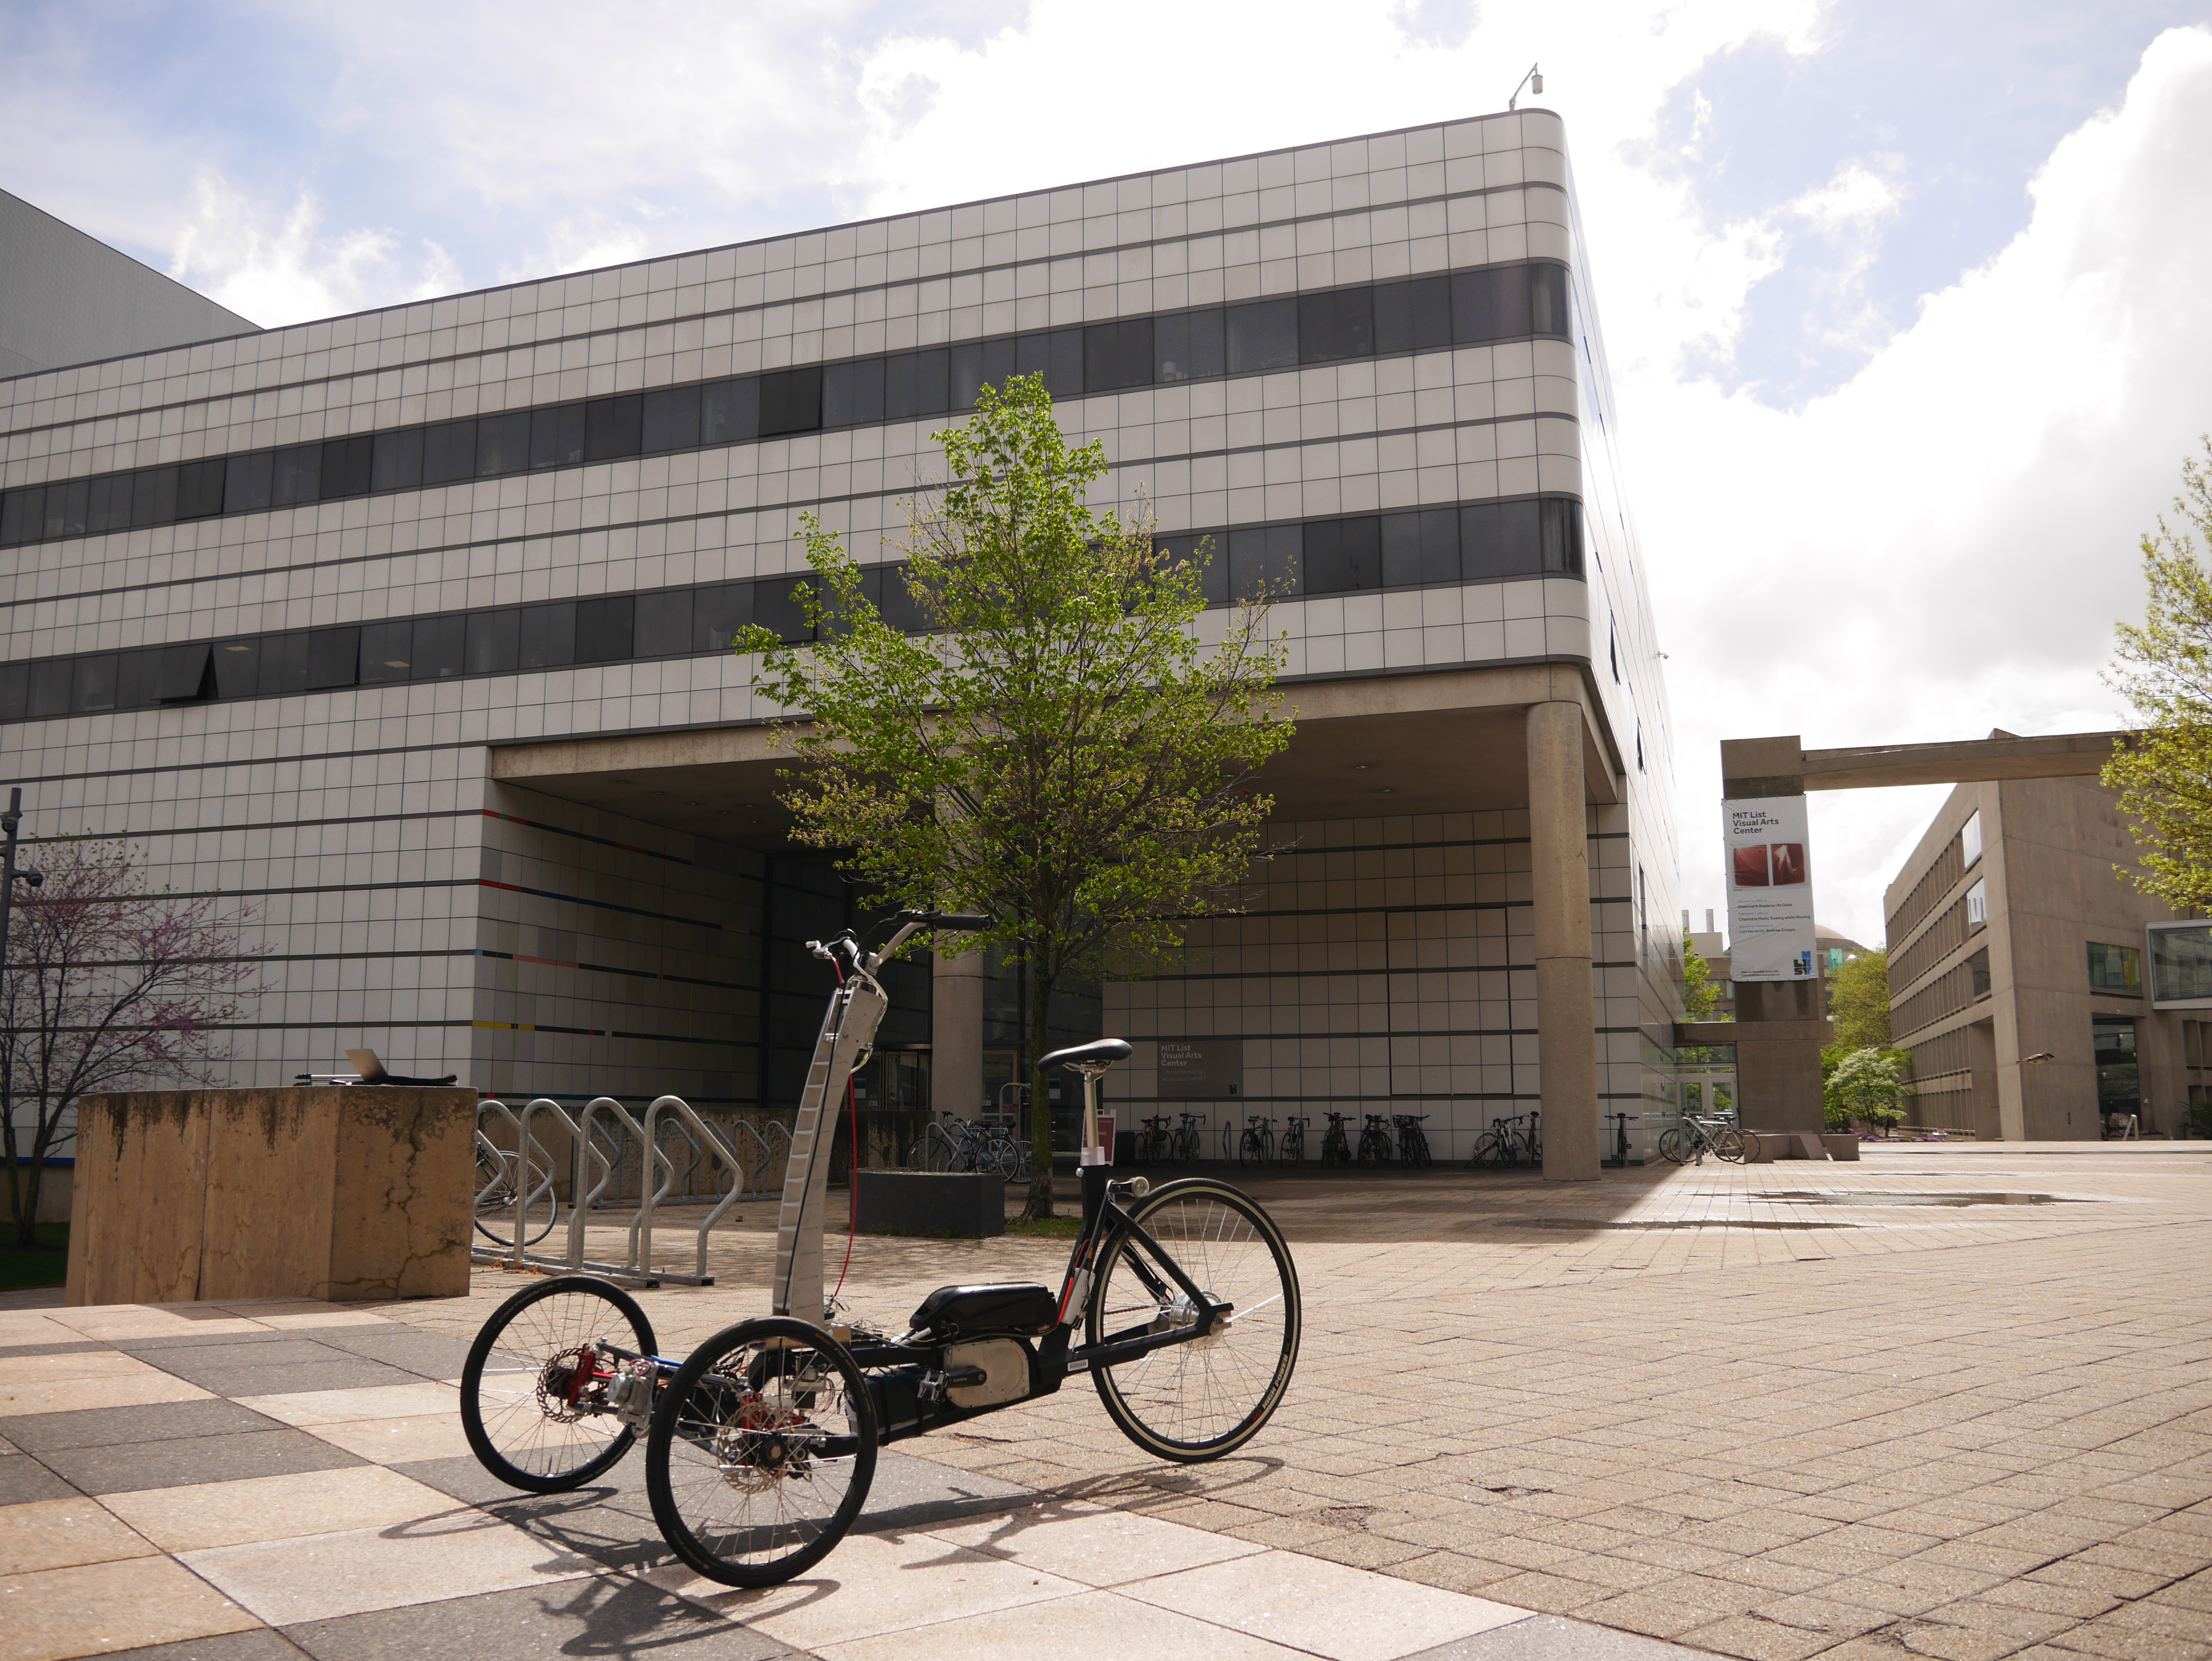
\includegraphics[width=1\linewidth]{figs/06/P1060127}
	\caption{PEV outside the MIT Media Lab}
	\\[-1.2cm]
\end{figure}
\subsection{Test Setup}

\begin{marginfigure}[6cm]
	\includegraphics[width=1\linewidth]{figs/06/circuit}
	\caption{Testing setup schematic}
\end{marginfigure}
With the intention of comparing the experimental results with the carried out simulations, the PEV was tested under some controlled conditions. The 6th floor of the MIT Media Lab was selected as the test field due to the available space and the accessibility of the room. The geometry of the experiment was limited by two circumferences of known radius ($R=2.5m$). These circumferences were delimited by some cardboard boxes laid on the floor.

As has been stated below, the first tests were run to validate the data coming from the sensors. The throttle potentiometer did not implicate any problem, neither did the rotary encoder at the rear wheel. On the contrary, the pair of IMUs (in the frame and in the handle bar) presented some problems.
\begin{itemize}
\begin{itemize}
\item In the calibration stage, the IMUs seemed to lose the 'north pole' every time the PEV was transported from one floor to another. However, when testing in the same floor, these problem did not appear. To solve this issue, the IMUs had to be calibrated again with each test. 

\item This calibration problem also affected considerably the initial absolute orientation of both IMUs, meaning that the relative angle between them --for the $\delta$ angle, for example-- had a initial drift.

\item The noise coming from the accelerometer and the gyroscope was excessive for a good control feedback. Each signal coming from the IMU was filtered with a simple one dimensional Kalman filter. Some preliminary tests were necessary to estimate the parameters of each Kalman filter: $p,\, q,\,k$.

\end{itemize}
\end{itemize}

The data was gathered using one of the Bluetooth modules, that sent the data to the computer, where the selected variables were saved in a .csv file. Afterwards, the data and the video from the front camera were a synchronized using an script in Matlab.

\begin{figure}[!h]
	\includegraphics[width=1\linewidth]{figs/06/live}
	\caption{Live streaming through Bluetooth module}
	\\[-1cm]
\end{figure}

The PEV was tested with and without the tilting mechanism, thanks to the modularity of the front suspension design. The non-tilting PEV was used for the tests where the sensor data was being validated and for the tests where the control strategy was implemented. After all the systems had been validated, the PEV was modified to allow the tilting and the final experiments were carried out.
 
\begin{figure*}[b]
	\includegraphics[width=1\linewidth]{figs/06/test_1}
	\caption{Testing setup}
	\\[-1.5cm]
\end{figure*}

\newpage

\subsection{Test Results}

The improvement of the PEV from the first to the last test was evident. The vehicle was exhaustively tested to improve the steering response as well as the remote control from the Android app. The mechanical robustness of the vehicle was put to the test during these experiments.

In the next set of pictures (Figure \ref{scene_2}), two turns to the circumference are illustrated. Before running any test, the PEV team consensually decided not to put in risk the integrity of any member, so it was decided to experiment only with driverless PEV. The main focus of these tests was the validation of the mechanics, the electronics and the control strategy. 

It is important to recall that at the test stage any false step can imply the breaking of the PEV or in the worst case scenario, the harm of the researches. A testing vehicle can suppose a danger if it gets out of control, so some safety measures, both at the hardware and the software level were implemented.

Therefore, since it was a driverless test, the PEV was remotely controlled, both at the steering and at the throttle. In this experiment, the control of the PEV was smooth, and the data was correctly gathered for the afterwards analysis.

With regards to the tilting mechanism, it successfully worked properly, meaning that the front suspension geometry was appropriate and that the selection of the components was satisfactory. In addition, the self limitation of the geometry limited the tilting angle to a maximum, thus preventing the PEV from rolling over when tilting.

\begin{figure*}[!h]
	\includegraphics[width=1\linewidth]{figs/06/scene_2}
	\caption{Testing scene}
	\label{scene_2}
\end{figure*}

\newpage

\begin{marginfigure}
	\includegraphics[width=1.15\linewidth]{figs/06/scene00151}
	\caption{PEV tilting during the test}
\end{marginfigure}
Even though the control strategy was not fully validated, the implementation of the feedback and feedforward gains showed that the torque $M_{t}$ was giving good inputs for the tilting.

The main problem with the control strategy was focused on the integration of the perceived lateral acceleration ($a_{per}^{I}$). The integration of a signal coming from the IMU was reviewed in the chapter 4, where the velocity of the MiniPEV was estimated from the longitudinal linear acceleration. The similarities between the two challenges seem obvious. That is why the control strategy had to be finally reduced to the output variable  $a_{per}$ instead of $a_{per}^{I}$

In figures \ref{Picture1},\ref{Picture2}, \ref{Picture3} and \ref{Picture4} a sample of the carried out test has been included. This experiment was carried out allowing the tilting of the vehicle, and the control strategy was almost similar to the one presented previously in this chapter. The only difference can be found in the output variable, that is the $a_{per}$ instead of $a_{per}^{I}$. 

As was already mentioned, lateral stability is obtained when $a_{per}=0$. The control of the integrated value of $a_{per}$ avoids the model errors due to parameters uncertainty, neglected dynamics or linearization of the model. Therefore, these are the errors that can appear if only the $a_{per}$ is controlled. In this case the process to obtain the gains is completely similar.

The Figure \ref{Picture1} represents the disturbance of the model, that is, the input from the driver. The steering angle indicates the desired direction. In this case, the vehicle does turn to the left before turning to the right. The reader can visualize the inherent noise in the steering rate $\dot{\delta}$. Even though the Kalman filter revokes some of the signal noise, it is important to remind that the gyroscope data is very prone to vibrations.
\begin{figure}[!h]
	\includegraphics[width=1\linewidth]{figs/06/tests/Picture1b}
	\caption{Disturbance signal; input from the driver $\delta$ and $\dot{\delta}$}
	\label{Picture1}
\end{figure}
\newpage

The velocity of the vehicle has been included in Figure \ref{Picture2}. This test was carried out at low speed, in order to have the vehicle under control if necessary. The lateral perceived acceleration $a_{per}$ is noisy as well, whereas the yaw rate $\dot{\psi}$ is more smooth. Anyway, the data confirms that both variables are properly calculated. 

Before any input from the driver --when the vehicle is going in a straight line-- both the $a_{per}$ and the $\dot{\psi}$ are null. Just when the driver turns the handle bar and steers the front wheels, the yaw rate starts to increase (meaning a left turn) and the perceived acceleration takes negative values synchronously. Just when the steering angle is changed to the opposite direction, these two signals invert their values.

\begin{figure}[!h]
	\includegraphics[width=1\linewidth]{figs/06/tests/Picture2b}
	\caption{Vehicle variables: longitudinal velocity, perceived lateral acceleration and yaw rate}
	\label{Picture2}
\end{figure}

The response of the control strategy is to apply a torque $M_{t}$ so that the effect of the disturbance $\delta$ on the perceived lateral acceleration $a_{per}$ is canceled. Using the gains calculated previously, the torque required from the tilting motor is represented in the Figure \ref{Picture4}. 

The control objective is obtained with very satisfying performances; $a_{per}$ does not exceed $1m/s^2$ and the maximum tilting torque value is 10 Nm. The fact that more torque is required to the right turn is due to the fact that the steering input is higher in this case, so that demanding more torque.
\begin{figure}[!h]
	\includegraphics[width=1\linewidth]{figs/06/tests/Picture4b}
	\caption{Torque required by the control system to tilt the PEV}
	\label{Picture4}
	\\[-3cm]
\end{figure}

\newpage
The applied torque in the tilting motor leans the PEV and as a consequence, there is a change in the tilting angle $\theta$ and in the tilting rate $\dot{\theta}$. In this case the maximum tilting angle goes over $0.15 rad=8 deg.$, which is not very high due to the low speed of the test.
 
\begin{figure}[!h]
	\includegraphics[width=1\linewidth]{figs/06/tests/Picture3b}
	\caption{Control strategy results}
	\label{Picture3}
\end{figure}

Overall, the carried out tests were satisfactory in almost every way. The exclusion of  the integrate of the perceived lateral acceleration from the control strategy changed the properties and the robustness of the system, but far from ruining the developed control model, this fact introduced a much simpler and effective model. While it is true that some errors can rise --parameters uncertainty, neglected dynamics or model linearization -- the reduced model successfully tilt the vehicle. 

%\begin{figure*}[!h]
%	\includegraphics[width=1\linewidth]{figs/06/tests/Picture5}
%	\caption{Control strategy results}
%	\label{Picture5}
%\end{figure*}

\begin{figure}[b]
	\includegraphics[width=1\linewidth]{figs/06/test_2}
	\caption{PEV testing}
\end{figure}



